%---------------------------------------------------------------------
%
%                          Capítulo 4 - Descripción del problema
%
%---------------------------------------------------------------------

\chapter{Termómetro de la ira}

En este capítulo se va a detallar el proceso que se ha seguido para llegar a implementar el termómetro de la ira. En la sección~\ref{sec:c4:intro} se introduce el problema al que se desea dar solución con el termómetro de la ira. En la sección~\ref{sec:c4:cap} se explica cómo se ha llevado a cabo la captura de requisitos y cuáles fueron los requisitos iniciales de la aplicación. En la sección~\ref{sec:c4:diseño} se explica cómo se desarrolló el diseño de la aplicación con la ayuda de los usuarios finales y la experta en el tratamiento de la ira. Por último, en la sección~\ref{sec:c4:impl}, se detalla cómo se ha implementado y se muestra el resultado final.

%-------------------------------------------------------------------
\section{Introducción}
\label{sec:c4:intro}
\paragraph{}
A la hora de tratar clínicamente a un paciente con problemas de salud mental, existe el problema de que aquello que cuenta el paciente sobre su problema puede no corresponderse con la realidad. Un paciente puede acudir por voluntad propia o de terceros y tanto su versión como la interpretación de los hechos que le han llevado a la consulta pueden diferir severamente entre cada persona. En el caso concreto de la ira, tal y como se comentaba en la sección~\ref{subsubsec:intervencionPsico}, la ira se desarrolla en entornos muy específicos (y diferentes entre cada paciente), supone una distorsión intencionada de la realidad y, por la deseabilidad social del paciente, puede que niegue que tenga problemas de gestión de la ira a la hora de dirigirse al terapeuta.

\paragraph{}
Por todo ello, se propone una solución tecnológica en la que, por un lado el paciente pueda tener en tiempo real información que le sea de utilidad para gestionar dicho episodio de ir y, por otro, dé información adicional a la terapeuta para guiar la consulta para la gestión de la ira. Se propone un sistema tecnológico que mida de forma continuada las constantes fisiológicas del paciente sin que esto interfiera en su día a día, interprete y detecte los episodios de ira y cuando surja un episodio de ira, la aplicación le dará una serie de pautas (previamente cargadas en el sistema por el terapeuta) que le ayuden a gestionar el episodio de ira para volver a una situación de calma. Toda la información del paciente se irá registrando para su posterior análisis por parte del terapeuta. La información recogida resultará de gran ayuda para detectar si el tratamiento está siendo efectivo (es decir, si los episodios de ira disminuyen en intensidad, duración y frecuencia a lo largo del tiempo) y si las pautas asignadas por el terapeuta son o no efectivas.

\paragraph{}
Para medir las constantes fisiológicas se utilizará una pulsera inteligente, que es un formato de dispositivo inteligente ampliamente usado entre segmentos muy diversos de la población, lo que evitará la estigmatización del paciente ya que nadie tiene por qué saber el uso que se está dando a la pulsera.

\paragraph{}
Es importante recalcar que esta solución tecnológica bajo ningún concepto pretende sustituir la terapia con el paciente. Por contra, es una herramienta adicional que intenta mejorar los resultados de la atención clínica al paciente en cuestión.

\paragraph{}
Debido a que no somos expertos en el tratamieto de la ira, en este proceso será fundamental realizar un diseño centrado en el usuario, en el que se contará en todas las fases del proceso con una persona experta que trabaja con la gestión de la ira.

\section{Captura de requisitos}
\label{sec:c4:cap}
\paragraph{}
Una vez identificado el problema, es fundamental establecer contacto con usuarios finales de la aplicación para capturar los requisitos. En este caso, existen dos perfiles de usuarios finales: los pacientes con ira disfuncional y los terapeutas de dichos pacientes. Para este caso, se ha incorporado el conocimiento de una psicóloga que trabaja con este tipo de pacientes que guiará el diseño no solo en lo que concierne a la información que le será útil al terapeuta sino también a qué y cómo debe presentarse la información a los pacientes con ira disfuncional.

\paragraph{}
Para la captura de requisitos, se han realizado dos reuniones con la psicóloga en las que se han recogido unos requisitos que tengan en cuenta tanto las necesidades de los usuario finales como las restricciones tecnológicas. Así, los requisitos funcionales que se han definido tras estas reuniones son:

\begin{enumerate}
    \item Una pulsera inteligente recogerá las constantes fisiológicas a partir de las cuales se intentará averiguar si dicho paciente está sufriendo ira.
    \item El paciente tendrá una aplicación instalada en su móvil, cuyo sistema operativo debe ser Android.
    \item El terapeuta tendrá una aplicación web donde podrá ver el registro de episodios de sus pacientes así como modificar las pautas asociadas a cada uno de ellos.
    \item Cuando se detecte que el paciente pueda estar sufriendo ira, en el móvil del paciente, deberán aparecerle pautas que le ayuden a gestionar dicha ira hasta que se detecte que el episodio ha terminado (el paciente ha vuelto a un estado de calma).
    \item El grado de ira que se le presentará al paciente en un termómetro horizontal en el que el menor valor esté a la izquierda y el valor de mayor ira esté a la derecha.
    \item El paciente podrá descartar pautas y emitir comentarios sobre las mismas para así poder afinar mejor las pautas que les son útiles a cada paciente.
    \item Se registrará el uso y desuso de las pautas para cada paciente, pudiendo el terapeuta modificarlas convenientemente si viese que estas no están siendo útiles.
    \item Todos los episodios de ira del paciente serán registrados para su posterior revisión por parte del terapeuta y del propio paciente.
    \item Las pautas deben de ser definidas por el terapeuta.
    \item La aplicación móvil para el paciente debe ser muy visual y con una curva de aprendizaje poco elevada, lo que implicará limitar el rango de acciones disponibles para el usuario.
    \item Los textos de la aplicación deberán ser en lectura fácil\footnote{Los textos de lectura fácil son aquellos que se realizan con un vocabulario sencillo para que estos puedan ser comprendidos por personas con discapacidad intelectual.} para que estos puedan ser accesibles para todo tipo de usuarios.
\end{enumerate}

\section{Diseño}
\label{sec:c4:diseño}
\paragraph{}
Una vez establecidos los requisitos que debe cumplir la aplicación, se definió la interfaz y las interacciones. El diseño se ha creado en dos iteracciones que se presentan en detalle en las siguientes subsecciones. En la primera iteracción se utilizaron prototipos en papel porque es una solución que requiere de poco esfuerzo temporal y es muy versátil, a la vez que es independiente de las tecnologías que luego se puedan usar. La ventaja de esto es que los cambios en esta etapa prematura del proceso no suponen una inversión elevada de tiempo en modificaciones del diseño.

\paragraph{}
En la segunda iteracción los prototipos que se presentaron fueron de alta fidelidad y se realizaron con las mismas tecnologías con las que luego se implementaría la solución, es decir, HTML y Android.

\subsection{Primer iteracción}
\paragraph{}
En los prototipos en papel, se incluían recortables de papel que al juntarlos entre sí, formaban las distintas pantallas de la web. Se intentó dar distintas alternativas para la misma funcionalidad o interacción aunque como se verá, existen algunos casos con una única opción. Esto se debe a que se creyó que la solución propuesta era estándar o no podía mejorarse significativamente con otras alternativas.

\subsubsection{Diseño de la aplicación móvil de los pacientes}

\paragraph{}
En la figura~\ref{fig:c4:mockup1} se muestra la pantalla que le aparecería al paciente nada más iniciar la aplicación. Es una pantalla de emparejamiento en la que el paciente tendría que introducir el token que le diera el terapeuta para así poder emparejar la aplicación con el paciente.

\paragraph{}
La pantalla de la figura~\ref{fig:c4:mockup2} es una alternativa a la pantalla~\ref{fig:c4:mockup1} pero con cadenas de caracteres de longitud tres. Más tarde se vio que esta pantalla ofrecía información duplicada respecto a la primera, por lo que en las siguientes versiones no se volvió a repetir su contenido.

\begin{figure}[h]
    \centering
    \begin{minipage}{.45\textwidth}
        \centering
        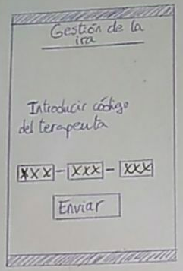
\includegraphics[width=0.8\linewidth, height=7cm]{Imagenes/anxA1-1.png}
        \caption[Mockup para iniciar sesión en la aplicación (versión I)]{Mockup para iniciar sesión en la aplicación (versión I)}
        \label{fig:c4:mockup1}
    \end{minipage}
    \hfill\vline\hfill
    \begin{minipage}{.45\textwidth}
        \centering
        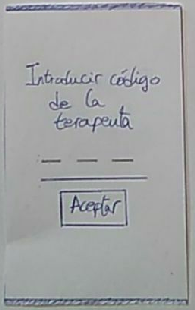
\includegraphics[width=0.8\linewidth, height=7cm]{Imagenes/anxA1-5.png}
        \caption[Mockup para iniciar sesión en la aplicación (versión II)]{Mockup para iniciar sesión en la aplicación (versión II)}
        \label{fig:c4:mockup2}
    \end{minipage}
\end{figure}

\paragraph{}
En la figura~\ref{fig:c4:mockup3}, aparece la pantalla con el nivel actual de ira del paciente. Si el paciente tiene un nivel de ira elevado (se encuentra inmerso en un episodio de ira) en esta pantalla también aparecen la pauta recomendada y la opción para introducir un comentario (por ejemplo, si decide no seguir la pauta recomendada).

\paragraph{}
La pantalla de la figura~\ref{fig:c4:mockup4} es una alternativa de las pantallas que aparecen en las figuras~\ref{fig:c4:mockup3},~\ref{fig:c4:mockup5} y~\ref{fig:c4:mockup6}, en el que la pantalla en la que aparece el nivel de ira y las pautas recomendadas se combina con la pantalla para sincronizar el dispositivo.

\begin{figure}[h]
    \centering
    \begin{minipage}{.4\textwidth}
        \centering
        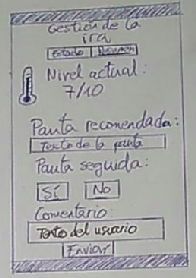
\includegraphics[width=0.8\linewidth, height=7cm]{Imagenes/anxA1-2.png}
        \caption[Mockup para ver el estado de ira y la pauta recomendada (versión II)]{Mockup para ver el estado de ira y la pauta recomendada (versión II)}
        \label{fig:c4:mockup3}
    \end{minipage}
    \hfill\vline\hfill
    \begin{minipage}{.4\textwidth}
        \centering
        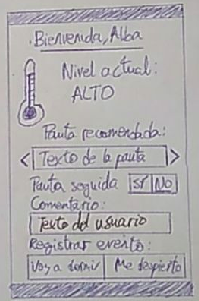
\includegraphics[width=0.8\linewidth, height=7cm]{Imagenes/anxA1-4.png}
        \caption[Mockup para ver el estado de ira y la pauta recomendada (versión I)]{Mockup para ver el estado de ira y la pauta recomendada (versión I)}
        \label{fig:c4:mockup4}
    \end{minipage}%
\end{figure}

\paragraph{}
En la figura~\ref{fig:c4:mockup5} aparece la pantalla para calibrar la pulsera en la que el paciente debe seleccionar si se va a dormir o a despertar. Una vez sincronizada la pulsera, esta pantalla ya no vuelve a aparecer. Esta pantalla es la única con la que podrá interactuar el usuario hasta que haya sincronizado el dispositivo, puesto que cada persona tiene unas constantes vitales distintas y sin esta información no es posible detectar los episodios de ira del paciente.

\paragraph{}
La pantalla de la figura~\ref{fig:c4:mockup6} es la segunda opción que se dio para la pantalla de la figura~\ref{fig:c4:mockup5}, cuya variación reside principalmente en darle al usuario la información de la hora a la que se acostó y se despertó para que así en caso de que haya sido introducido por error, esta información le ayude a dilucidarlo.

\begin{figure}[h]
    \centering
    \begin{minipage}{.4\textwidth}
        \centering
        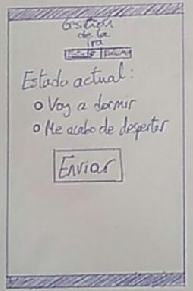
\includegraphics[width=0.8\linewidth, height=7cm]{Imagenes/anxA1-3.png}
        \caption[Mockup para calibrar el dispositivo (versión I)]{Mockup para calibrar el dispositivo (versión I)}
        \label{fig:c4:mockup5}
    \end{minipage}
    \hfill\vline\hfill
    \begin{minipage}{.4\textwidth}
        \centering
        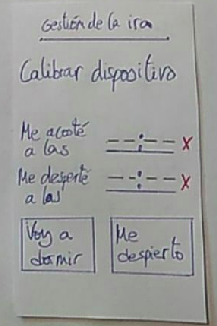
\includegraphics[width=0.8\linewidth, height=7cm]{Imagenes/anxA1-6.png}
        \caption[Mockup para calibrar el dispositivo (versión I)]{Mockup para calibrar el dispositivo (versión I)}
        \label{fig:c4:mockup6}
    \end{minipage}
\end{figure}

\paragraph{}
Una vez creados los prototipos en papel, se fijó una reunión con la psicóloga en la que se presentaron las distintas alternativas. Las principales conclusiones que se obtuvo de esta reunión fueron las siguientes:
\begin{itemize}
    \item La manera de emparejar la pulsera y el paciente que aparece en la figura~\ref{fig:c4:mockup2} es apropiada.
    \item Las dos alternativas para calibrar el dispositivo que se observan en las figuras~\ref{fig:mock5} y~\ref{fig:mock6} son apropiadas. No ve ninguna razón de peso para elegir una u otra, por lo que finalmente se optó por la alternativa de la figura~\ref{fig:c4:mockup6}, ya que le facilita más información al usuario y le permite rectificar la acción si pulsó accidentalmente alguno de los botones de la pantalla.
    \item El termómetro es una buena opción deberá aparecer en horizontal, estando el menor nivel de ira a la izquierda y el mayor en el otro extremo del termómetro, siguiendo la direccionalidad de la lectura en castellano.
    \item Para indicar el grado de ira, es mejor hacerlo con palabras (como en la figura~\ref{fig:c4:mockup2}) que de manera numérica (como en la figura~\ref{fig:c4:mockup1}). Los estados que discreticen el grado de ira que verá el paciente deberán ser reducidos para que el paciente pueda identificar su ordinalidad con facilidad. Así, la solución se limitará a cinco estados.
    \item Cuando varíe el grado de ira en el termómetro, no solo debe variar cuánto de lleno se encuentra éste, sino también su color. La terapeuta indicó que, tal y como comenta Valdez (\citeyear{valdez1994effects}), existe una relación estrecha entre emociones y colores, por lo que establecer por ejemplo que el rojo es el estado de calma y el verde es el estado de mayor percepción de la ira es un cambio significativo respecto a la asociación opuesta. En estudios experimentales se ha podido comprobar que los colores de mayor longitud de onda como son el rojo o el amarillo provocan mayor activación que otros de menor longitud de onda como es el verde. A su vez, Jacobs y Sues (\citeyear{jacobs1975effects}) han comprobado en un estudio con los colores rojo, amarillo, verde y azul que existe una mayor asociación del estrés con los colores rojo y amarillo respecto al verde y el azul. Así, a la hora de representar los colores asociados a cada nivel de ira, los colores asociados a estos niveles deberían ser (de menor a mayor nivel de ira): verde, verde-amarillo, amarillo, amarillo-rojo, rojo.
    \item Es importante que el paciente pueda cambiar de pauta si esta no le es útil.
    \item El comentario de las pautas debe ser opcional y se debe poder añadir usando la voz.
    \item Se deben incluir elementos sonoros que incrementen su volumen en función del nivel de ira del paciente para que este pueda ser consciente de que ha aumentado su nivel de ira.
    \item En la pantalla de la gestión de la ira se debe permitir al paciente seleccionar el tipo de situación que ha generado la ira.
\end{itemize}

\subsubsection{Diseño de la aplicación web del terapeuta}

\paragraph{}
El elemento de la figura~\ref{fig:c4:mockup7} sirve para mostrar cómo sería el inicio de sesión.

\paragraph{}
El elemento de la figura~\ref{fig:c4:mockup8} muestra una pantalla estándar para registrar a un paciente. El combo para seleccionar el grupo finalmente fue descartado.

\paragraph{}
El elemento de la figura~\ref{fig:c4:mockup9} muestra cómo se crearían grupos y se modificaría su composición de pacientes.

\paragraph{}
En las figuras~\ref{fig:c4:mockup10} y~\ref{fig:c4:mockup11} se muestran dos alternativas para mostrar las pautas: una única tabla para todos los niveles de activación en la que se cuenta con una columna del porcentaje de efectividad general entre los pacientes y una segunda con el texto de la pauta. La primera opción es más visual y cuenta con menos información: no se incluye la columna del porcentaje de éxito de cada pauta y las pautas están divididas en tablas según el nivel de activación asociado.

\begin{figure}[h]
    \centering
    \begin{minipage}{.4\textwidth}
        \centering
        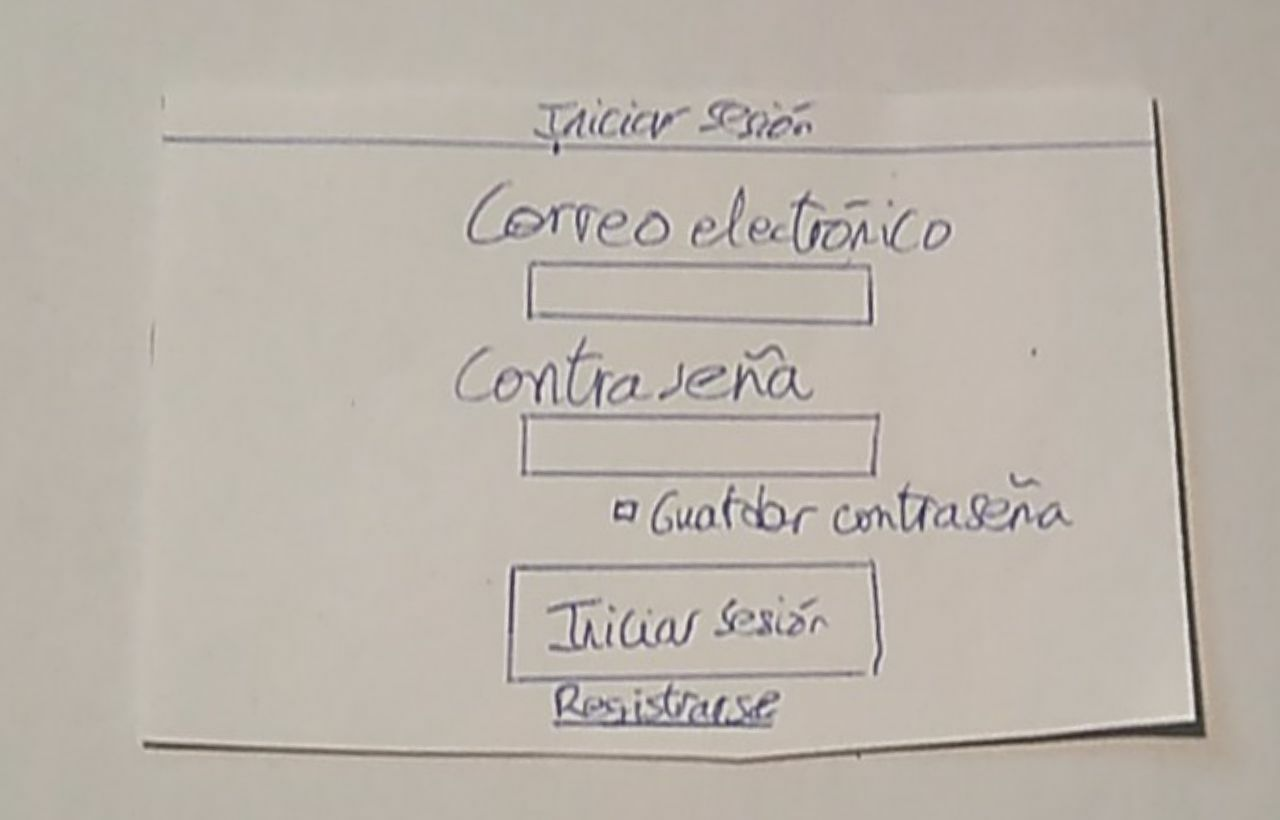
\includegraphics[width=0.8\linewidth, height=7cm]{Imagenes/anxA2.jpg}
        \caption[Mockup para iniciar sesión en la web]{Mockup para iniciar sesión en la web}
        \label{fig:c4:mockup7}
    \end{minipage}
    \hfill\vline\hfill
    \begin{minipage}{.4\textwidth}
        \centering
        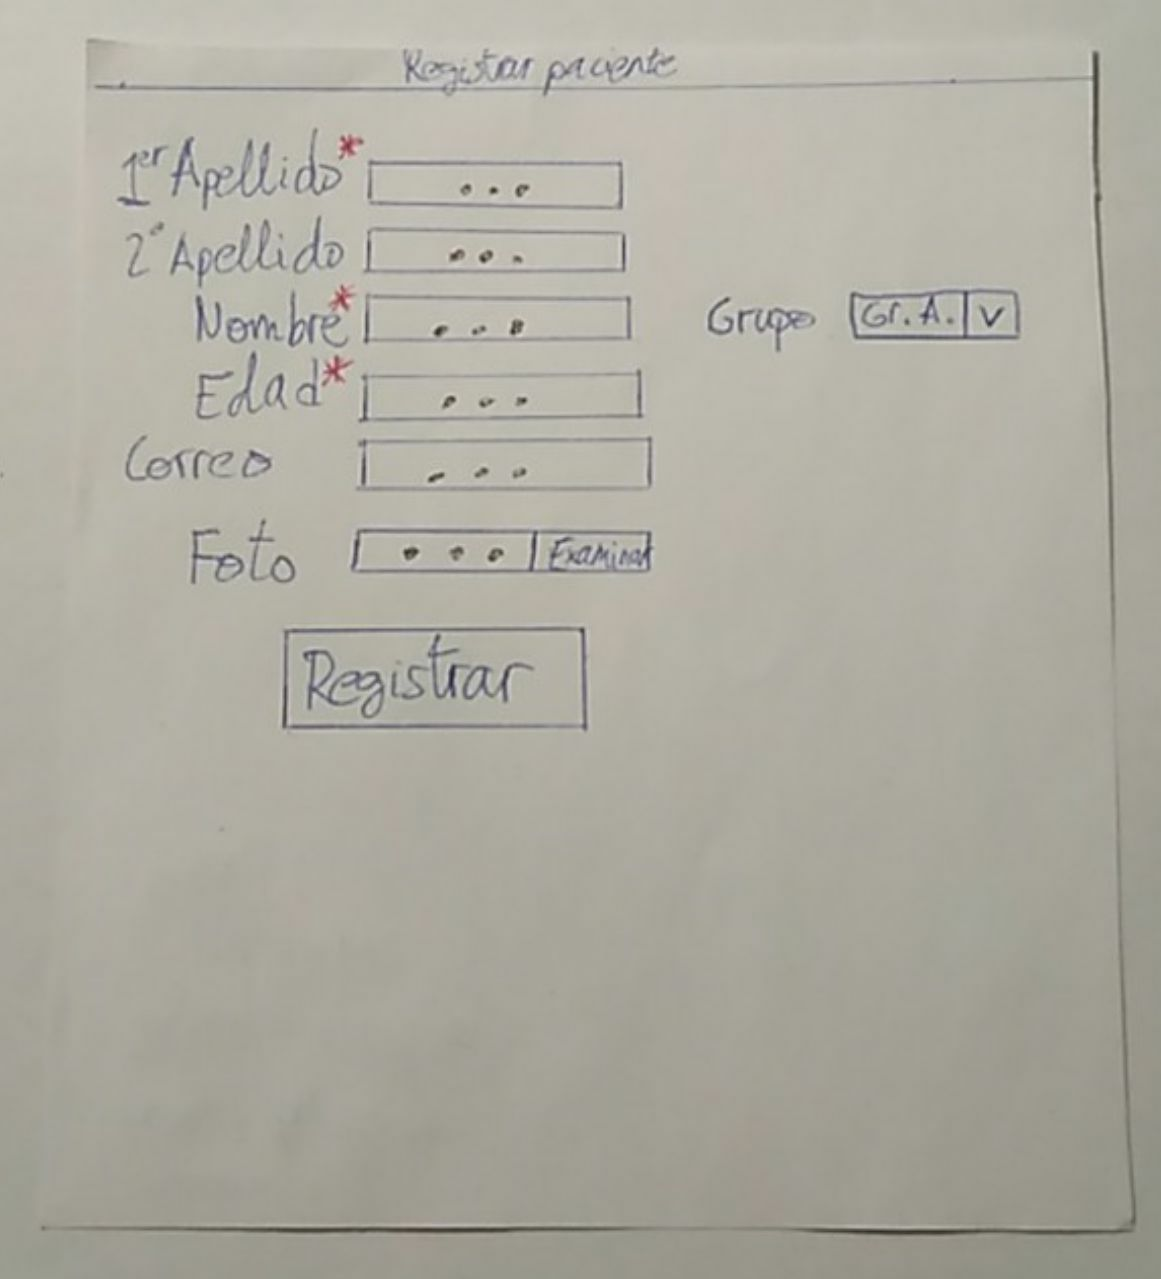
\includegraphics[width=0.8\linewidth, height=7cm]{Imagenes/anxA3.jpg}
        \caption[Mockup para registrar al paciente en la web]{Mockup para registrar al paciente en la web}
        \label{fig:c4:mockup8}
    \end{minipage}
\end{figure}

\paragraph{}
En la figura~\ref{fig:c4:mockup12} aparece una pantalla genérica para modificar el paciente en la que a su vez aparece la información asociada a las pautas que le han ido apareciendo en la aplicación móvil.

\paragraph{}
En las figuras~\ref{fig:c4:mockup13},~\ref{fig:c4:mockup14} y~\ref{fig:c4:mockup15} aparecen las tres opciones que se presentaban a la terapeuta para cada paciente en el que se podía ver el resumen de episodios de cada paciente. Dos de ellos consisten en tablas en las que en una aparece las pautas que se recomendaban y en el otro si la pauta suministrada funcionó o no. La opción alternativa era mostrar una gráfica con los distintos episodios acaecidos en un periodo de tiempo.


\begin{figure}[h]
    \centering
    \begin{minipage}{.45\textwidth}
        \centering
        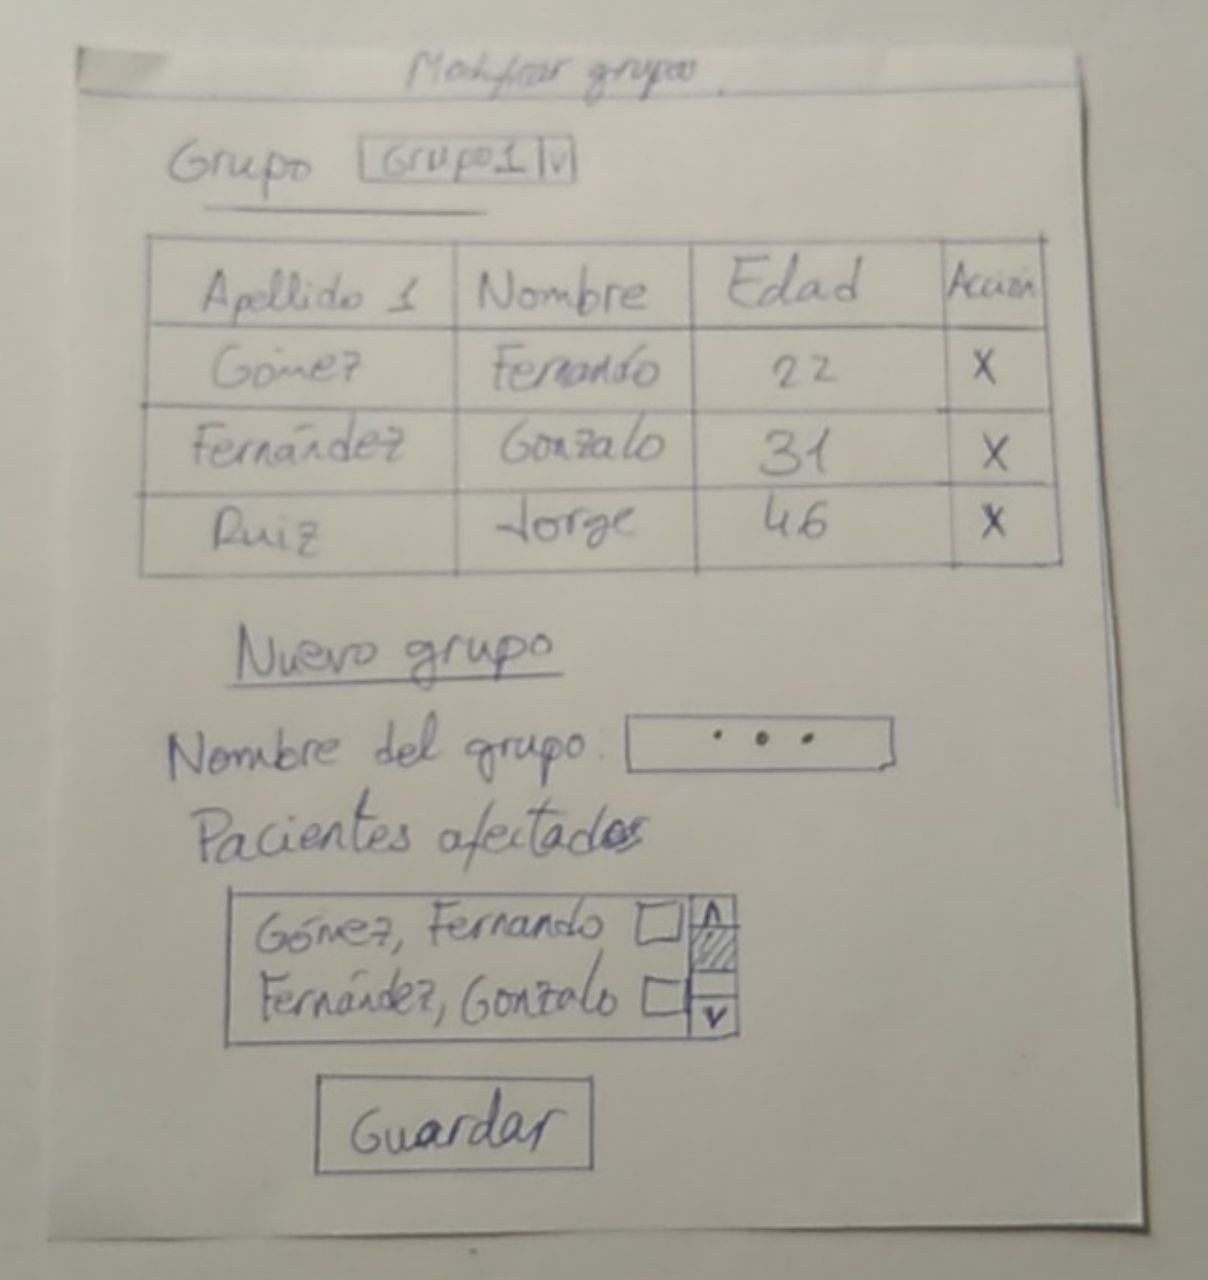
\includegraphics[width=0.8\linewidth, height=7cm]{Imagenes/anxA4.jpg}
        \caption[Mockup para la gestión de grupos de pacientes]{Mockup para la gestión de grupos de pacientes}
        \label{fig:c4:mockup9}
    \end{minipage}
    \hfill\vline\hfill
    \begin{minipage}{.45\textwidth}
        \centering
        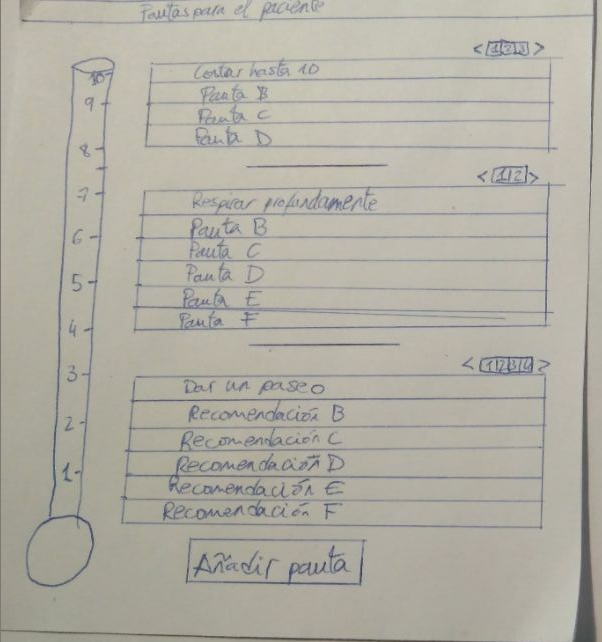
\includegraphics[width=0.8\linewidth, height=7cm]{Imagenes/anxA5-1.png}
        \caption[Mockup para la gestión de pautas (versión I)]{Mockup para la gestión de pautas (versión I)}
        \label{fig:c4:mockup10}
    \end{minipage}
\end{figure}

\paragraph{}
En la figura~\ref{fig:c4:mockup16} aparece un elemento genérico para incluir en la cabecera de la pantalla del usuario con información básica sobre este. Al pulsar sobre el botón modificar, se redireccionaría la a pantalla de la figura~\ref{fig:c4:mockup12}.

\begin{figure}[h]
    \centering
    \begin{minipage}{.45\textwidth}
        \centering
        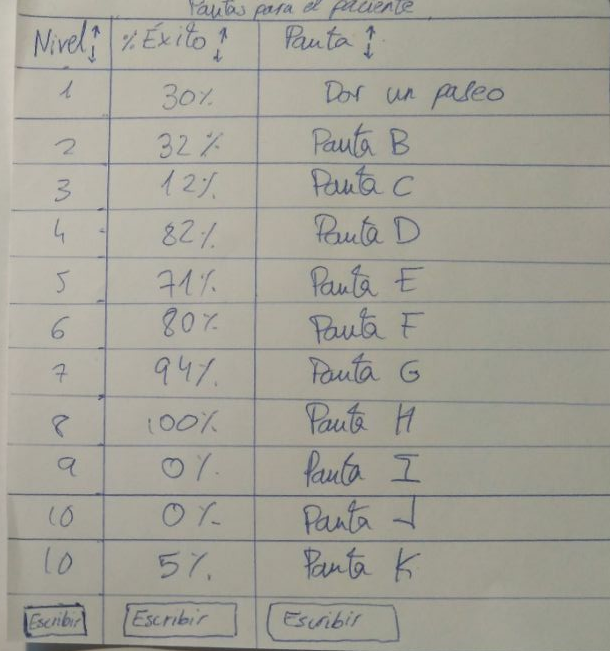
\includegraphics[width=0.8\linewidth, height=7cm]{Imagenes/anxA5-2.png}
        \caption[Mockup para la gestión de pautas (versión II)]{Mockup para la gestión de pautas (versión II)}
        \label{fig:c4:mockup11}
    \end{minipage}
    \hfill\vline\hfill
    \begin{minipage}{.45\textwidth}
        \centering
        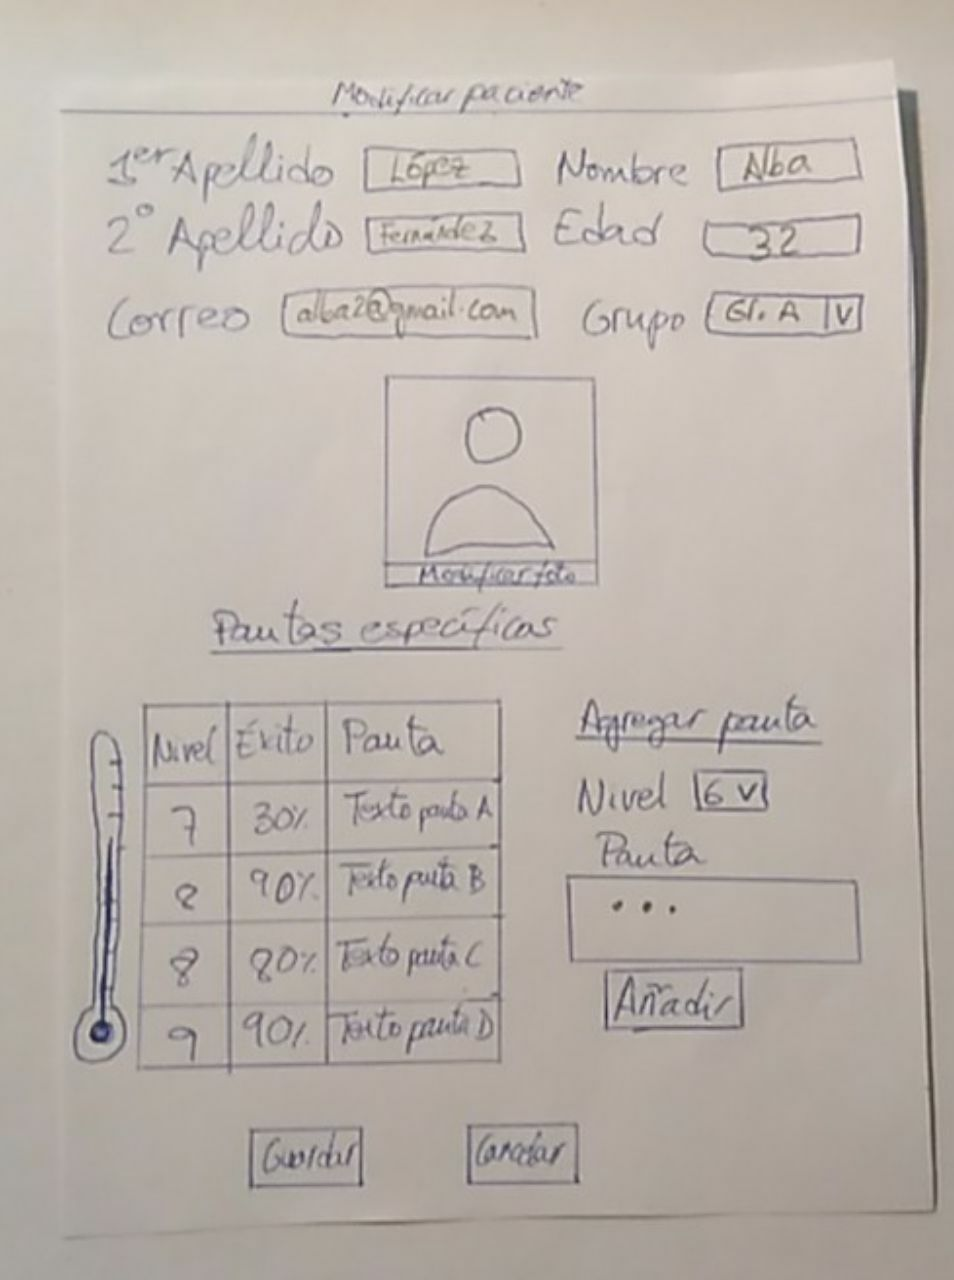
\includegraphics[width=0.8\linewidth, height=7cm]{Imagenes/anxA6.jpg}
        \caption[Mockup para la gestión de un paciente]{Mockup para la gestión de un paciente}
        \label{fig:c4:mockup12}
    \end{minipage}
\end{figure}

\paragraph{}
En la figura~\ref{fig:c4:mockup17} aparecen los dos elementos que se utilizarían tanto en la pantalla principal con el resumen de alertas de todos los pacientes como en la pantalla particular de cada paciente. El botón \textit{ver detalles} llevaría a una tabla o gráfica con el resumen de episodios citados.

\paragraph{}
En la figura~\ref{fig:c4:mockup18} aparece el resumen de los episodios de todos los pacientes en el periodo especificado en el segundo elemento de la figura anterior. Así, el elemento más a la izquierda sería un filtro de pacientes similar al que se encuentra en páginas web de compra de artículos en la que se podría filtrar a los mismos en función de la información que se tiene de ellos, así como se podría hacer usando el buscador horizontal que se encuentra en la parte superior de la imagen. Al pulsar sobre cualquiera de estas filas, se abriría la página con el resumen de episodios del paciente seleccionado. La diferencia entre ambas tablas reside principalmente en la utilización del espacio y en que la información provista sea menos o más visual: la opción más a la izquierda, a diferencia de lo que ocurre con la opción de la derecha, no incluiría fotografía y estaría pensada para ocupar menos espacio vertical por registro, lo que permitiría poder representar más registros en el mismo espacio respecto a la segunda opción.

\begin{figure}
    \centering
    \begin{minipage}{.45\textwidth}
        \centering
        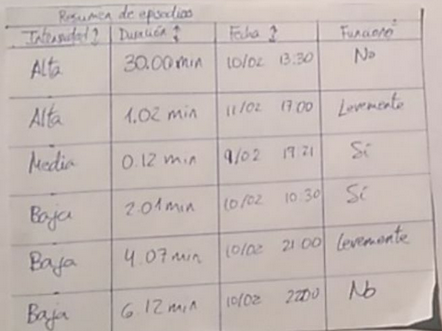
\includegraphics[width=0.8\linewidth, height=7cm]{Imagenes/anxA7-1.png}
        \caption[Mockup para mostrar los episodios de un paciente (versión I)]{Mockup para mostrar los episodios de un paciente (versión I)}
        \label{fig:c4:mockup13}
    \end{minipage}
    \hfill\vline\hfill
    \begin{minipage}{.45\textwidth}
        \centering
        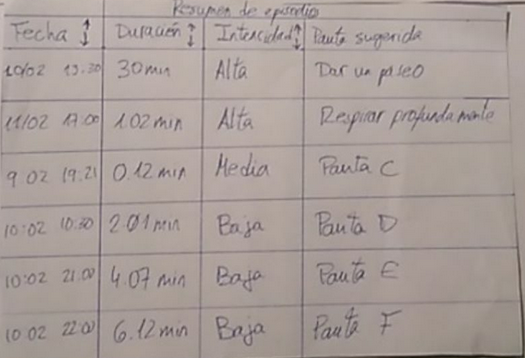
\includegraphics[width=0.8\linewidth, height=7cm]{Imagenes/anxA7-2.png}
        \caption[Mockup para mostrar los episodios de un paciente (versión II)]{Mockup para mostrar los episodios de un paciente (versión II)}
        \label{fig:c4:mockup14}
    \end{minipage}
\end{figure}

\paragraph{}
En la figura~\ref{fig:c4:mockup17} aparece el resumen de los episodios para todos los pacientes. Esto se incluiría en la página principal. La información es la misma, lo único que varía es su representación.

\begin{figure}
    \centering
    \begin{minipage}{.45\textwidth}
        \centering
        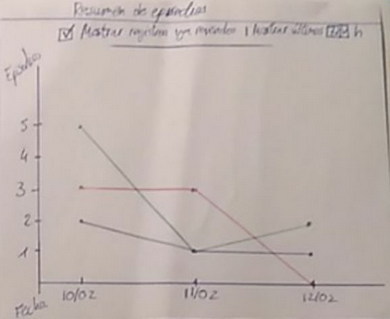
\includegraphics[width=0.8\linewidth, height=7cm]{Imagenes/anxA7-3.png}
        \caption[Mockup para mostrar los episodios de un paciente (versión III)]{Mockup para mostrar los episodios de un paciente (versión III)}
        \label{fig:c4:mockup15}
    \end{minipage}
\end{figure}


\begin{figure}[!htbp]
    \centering
    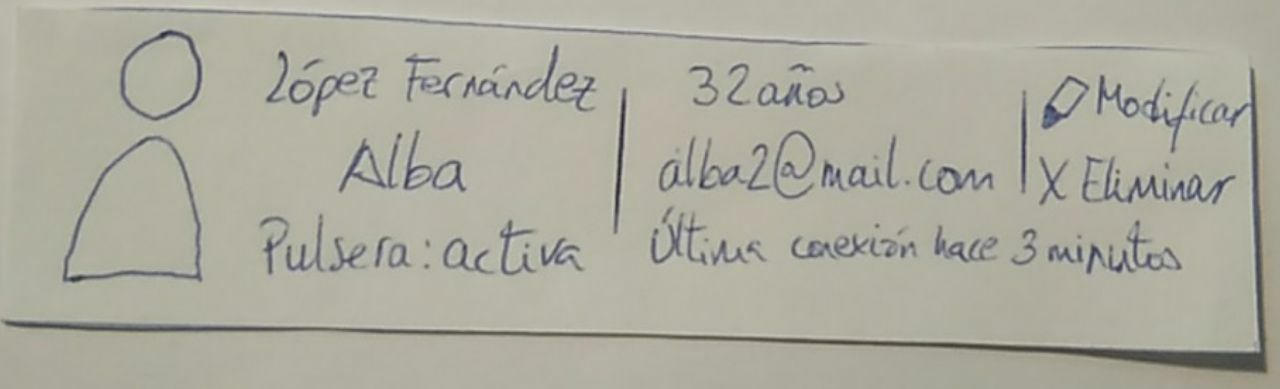
\includegraphics[scale=0.3]{Imagenes/anxA8.jpg}
    \caption[Mockup para mostrar la información básica del paciente]{Mockup para mostrar la información básica del paciente}
    \label{fig:c4:mockup16}
\end{figure}

\begin{figure}[!htbp]
    \centering
    %width=3cm, height=3cm
\begin{frame}{Frame Title}
    
\end{frame}[]    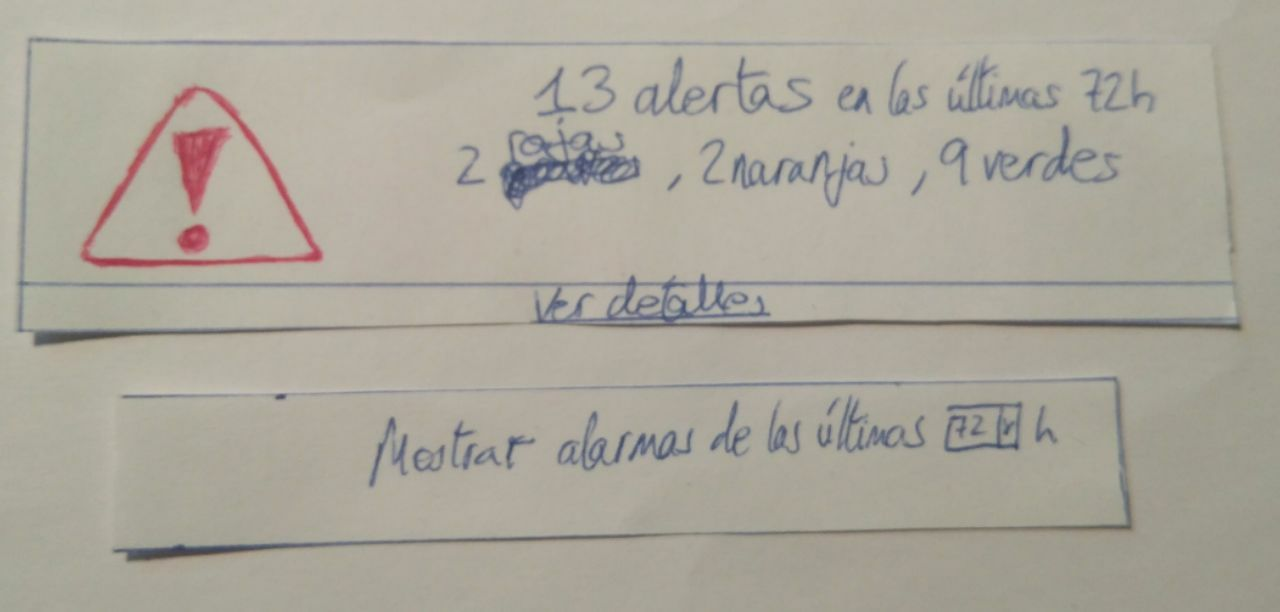
\includegraphics[scale=0.3]{Imagenes/anxA9.jpg}
    \caption[Mockup mostrar alertas de episodios de ira]{Mockup mostrar alertas de episodios de ira}
    \label{fig:c4:mockup17}
\end{figure}

\begin{figure}[!htbp]
    \centering
    %width=3cm, height=3cm
    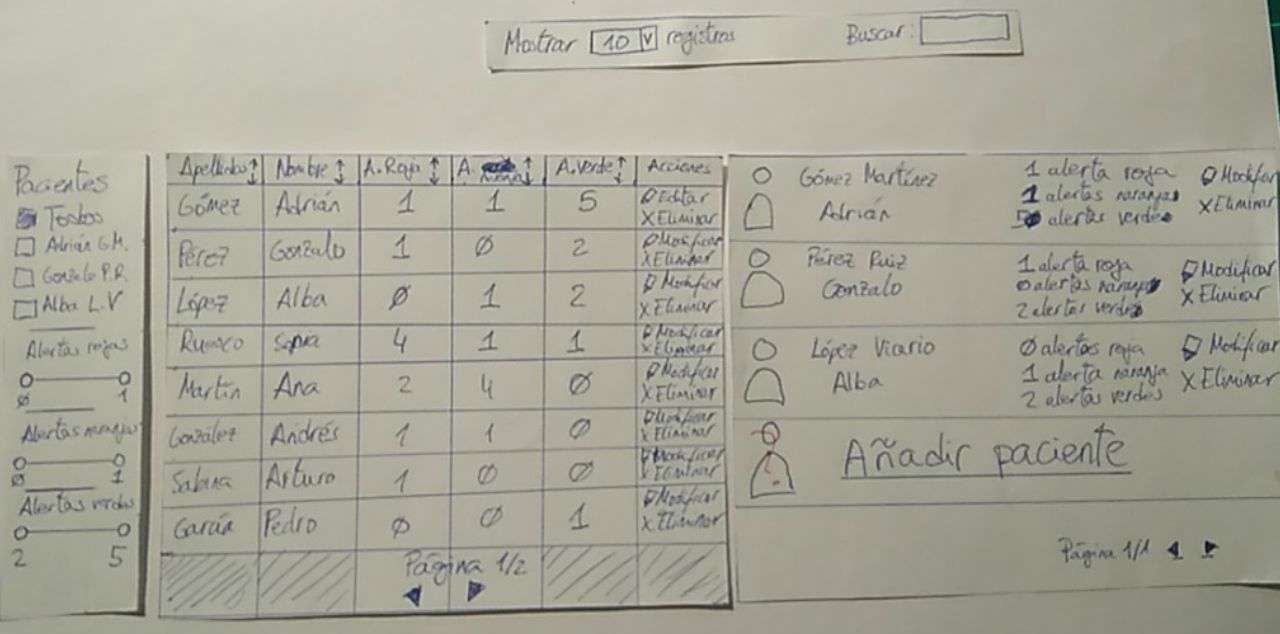
\includegraphics[scale=0.3]{Imagenes/anxA10.jpg}
    \caption[Mockup para mostrar los filtros y las dos opciones para mostrar la tabla de pacientes]{Mockup para mostrar los filtros y las dos opciones para mostrar la tabla de pacientes}
    \label{fig:c4:mockup18}
\end{figure}

\begin{figure}
    \centering
    \begin{minipage}{.45\textwidth}
        \centering
        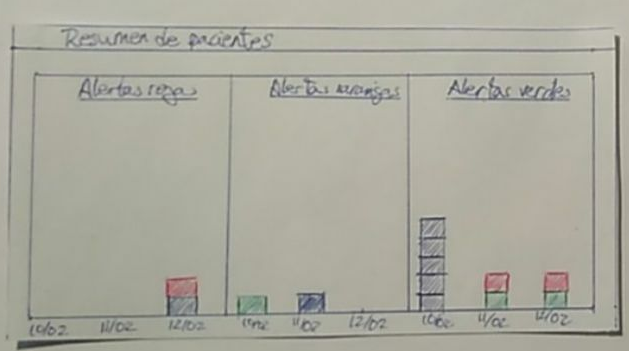
\includegraphics[width=0.8\linewidth, height=7cm]{Imagenes/anxA11-1.png}
        \caption[Mockup para mostrar el resumen de alertas de los pacientes (versión I)]{Mockup para mostrar el resumen de alertas de los pacientes (versión I)}
        \label{fig:c4:mockup19}
    \end{minipage}
    \hfill\vline\hfill
    \begin{minipage}{.45\textwidth}
        \centering
        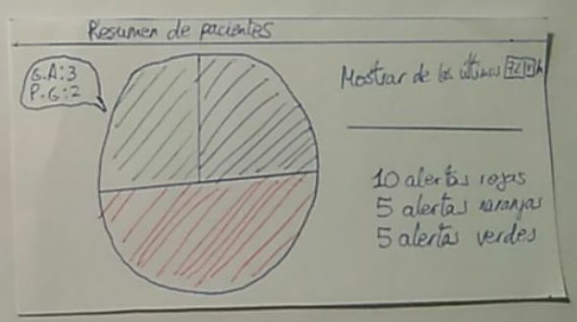
\includegraphics[width=0.8\linewidth, height=7cm]{Imagenes/anxA11-2.png}
        \caption[Mockup para mostrar el resumen de alertas de los pacientes (versión II)]{Mockup para mostrar el resumen de alertas de los pacientes (versión II)}
        \label{fig:c4:mockup20}
    \end{minipage}
\end{figure}

\paragraph{}
Una vez creados los prototipos en papel de la aplicación web, nos reunimos con la terapeuta para mostrarselos y buscar el diseño que mejor se ajustase a las necesidades de los usuarios finales. Las principales conclusiones que se obtuvo de esta reunión fueron las siguientes:

\begin{itemize}
    \item El método de autentificación del terapeuta para iniciar sesión con la tupla correo electrónico y contraseña es apropiado.
    \item A la hora de registrar un paciente,es apropiado poder incluir las fotos de pacientes para mejorar la visualización. El correo electrónico no es necesario y el grupo al que pertenece cada paciente es prescindible. Para futuras versiones podría ser interesante agrupar a los pacientes y obtener resultados globales de estos grupos pero para esta versión se acaba decidiendo que es mejor centrarse en una solución más sencilla. Por ello, la figura~\ref{fig:c4:mockup3} debe suprimir la selección del grupo y la pantalla de la figura~\ref{fig:c4:mockup4} no tiene que aparecer.
    \item Entre el primer y segundo elemento de la figura~\ref{fig:c4:mockup18} para representar las pautas de cada paciente, se considera que la solución tiene que ser algo intermedio: conservar la estructura del primer elemento de dividir las pautas en diversas tablas según su grado de intensidad (con un termómetro en paralelo para poder correlacionar fácilmente la intensidad de cada pauta) pero añadiendo columnas adicionales a las pautas como por ejemplo el porcentaje de éxito, tal y como se ve en el segundo elemento.
    \item Se considera apropiado que en el resumen de los episodios de ira figure el tiempo que se mantuvo el paciente en cada uno de los estados, tal y como aparece en el primer elemento de la figura~\ref{fig:c4:mockup14}.
    \item La información de la pauta recomendada para cada episodio, tal y como aparece en el tercer elemento de la figura~\ref{fig:c4:mockup14} se considera apropiada, pero es incompleto, ya que para un mismo estado al paciente se le puede haber recomendado más de una pauta. El paciente puede haber descartado pautas previas, y esta información es importante que quede registrada.
    \item La figura~\ref{fig:c4:mockup15} muestra la representación los episodios en formato histograma, lo que es correcto. El gráfico de tarta que aparece en la gráfica ~\ref{fig:c4:mockup20} no aporta información útil, porque cómo se ha desarrollado el episodio es relevante, como por ejemplo el tiempo que ha pasado en cada estado. El segundo elemento de la figura~\ref{fig:c4:mockup7} hace una aproximación a esto pero es incompleto, puesto que es necesario que sea una gráfica interactiva que permita poder ampliarla para por ejemplo poder seleccionar solo un episodio e ir viéndolos uno a uno. Para este fin, la terapeuta propone basarse en el ejemplo de las gráficas de los desfibriladores.
    \item Las figuras~\ref{fig:c4:mockup17} y ~\ref{fig:c4:mockup18} son elementos adicionales que sirven para decorar las pantallas que se iban generando. La figura~\ref{fig:c4:mockup17} se considera apropiada mientras que el primer elemento de la figura~\ref{mockup18} se considera que no aporta información útil para la terapeuta.
    \item En la figura~\ref{fig:c4:mockup19} aparecen dos modelos de tablas y una serie de filtros para poder buscar los pacientes en dichas tablas. Los filtros se consideran apropiados, y ambos formatos de tablas también a excepción de las columnas que indican el número de alertas de cada una de las intensidades de la ira de cada paciente, ya que esta información sin estar agrupada en episodios y desglosada en fechas, no aporta información relevante al terapeuta.
\end{itemize}

\subsection{Segunda iteracción}

\paragraph{}
Para esta segunda iteracción, se usaron prototipos de alta fidelidad con Android y HTML para que estos fueran lo más similares posibles al resultado final de la aplicación. Esto se debe a que, tras la primera iteracción, se pudieron extraer los suficientes requisitos como para poder avanzar en detalles más concretos de la aplicación final.

\subsubsection{Diseño de la aplicación móvil de los pacientes}

\paragraph{}
Las pantallas de esta segunda fase para el móvil son las siguientes:

\begin{itemize}
    \item En la figura~\ref{fig:c4:mockup21} aparece la pantalla para introducir el código para sincronizar la pulsera y el móvil con el paciente. Es la equivalente de la fase anterior que aparece en la figura~\ref{fig:c4:mockup1}.
    \item En la figura~\ref{fig:c4:mockup22} podemos ver la pantalla para sincronizar el dispositivo durante su primer uso.
\end{itemize}

\begin{figure}[h]
    \centering
    \begin{minipage}{.45\textwidth}
        \centering
        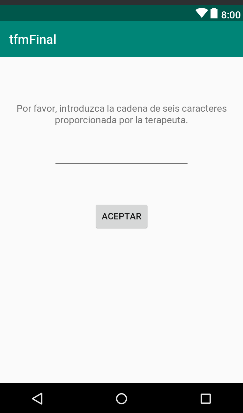
\includegraphics[width=0.8\linewidth, height=7cm]{Imagenes/anxA12.png}
        \caption[Mockup para sincronizar el dispositivo]{Mockup para sincronizar el dispositivo}
        \label{fig:c4:mockup21}
    \end{minipage}
    \hfill\vline\hfill
    \begin{minipage}{.45\textwidth}
        \centering
        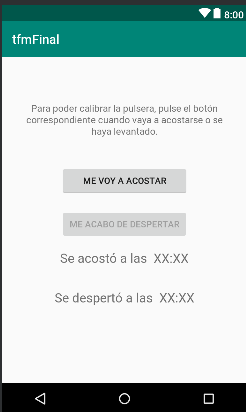
\includegraphics[width=0.8\linewidth, height=7cm]{Imagenes/anxA13.png}
        \caption[Mockup para calibrar el dispositivo]{Mockup para calibrar el dispositivo}
        \label{fig:c4:mockup22}
    \end{minipage}
\end{figure}

\begin{itemize}
    \item En la figura~\ref{fig:c4:mockup21} encontramos la que será la pantalla principal, donde aparece la pauta recomendada, el nivel de la ira representado mediante un termómetro horizontal, la posibilidad de cambiar de pauta y de enviar comentarios sobre la pauta en cuestión.
\end{itemize}

\begin{figure}[h]
    \centering
    \begin{minipage}{.45\textwidth}
        \centering
        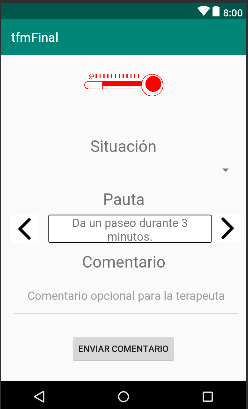
\includegraphics[width=0.8\linewidth, height=7cm]{Imagenes/anxA14.png}
        \caption[Mockup de la pantalla principal]{Mockup de la pantalla principal}
        \label{fig:c4:mockup23}
    \end{minipage}
    \hfill\vline\hfill
    \begin{minipage}{.45\textwidth}
        \centering
        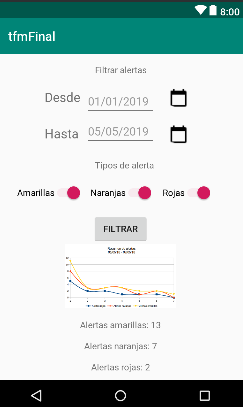
\includegraphics[width=0.8\linewidth, height=7cm]{Imagenes/anxA15.png}
        \caption[Mockup del histórico de episodios de un paciente]{Mockup del histórico de episodios de un paciente}
        \label{fig:c4:mockup24}
    \end{minipage}
\end{figure}

\begin{itemize}

    \item En la figura~\ref{fig:c4:mockup24} se encuentra una pantalla de resumen de la evolución seguida por el paciente. Esto es una innovación respecto a la anterior versión puesto que la terapeuta comentó que esta información puede servir para motivar al paciente al poder verificar en un histograma cómo se han reducido sus episodios de ira.

\begin{figure}[h!]
    \centering
    \begin{minipage}{.45\textwidth}
        \centering
        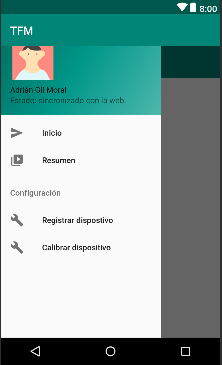
\includegraphics[width=0.8\linewidth, height=7cm]{Imagenes/anxA16.png}
        \caption[Mockup del menú de la aplicación]{Mockup del menú de la aplicación}
        \label{fig:c4:mockup25}
    \end{minipage}
\end{figure}

    \item En la figura~\ref{fig:c4:mockup25} se puede ver la manera que se utilizaría para cambiar entre las pantallas. En lugar de tener un menú horizontal que quite espacio para el resto de pantallas, este menú se desplegará como se hace en aplicaciones como Telegram o Whatsapp mediante el pulsado en un bocadillo a la izquierda de la barra horizontal superior o mediante el desplazamiento de la pantalla de izquierda a derecha.
\end{itemize}

\paragraph{}
Al revisar este diseño con la terapeuta, se obtuvieron las siguientes conclusiones:

\begin{itemize}
    \item Las pantallas que se muestran se ajustan bastante a lo esperado por parte de la terapeuta, pero en ellas aparece el concepto de alertas que debe desaparecer. Un episodio es un conjunto cronológicamente ordenado de alertas que empieza en el estado de reposo y acaba en el estado de reposo. Esa debe ser la unidad mínima con la que el terapeuta debe trabajar.
    \item El termómetro de la imágen debe ir al revés: el elemento de mayor grosor tiene que ir a la izquierda, que representará el menor nivel de ira.
    \item Se debe incluir un widget en la aplicación en el que aparezca un pequeño termómetro con el nivel de ira del paciente en ese momento para que el paciente pueda ver su estado actual de la ira sin necesidad de abrir la aplicación.
    \item Se deben incluir mensajes de alertas motivacionales tipo \textit{toast} como refuerzo positivo para el paciente cuando se detecte una disminución continuada de sus episodios de ira.
    \item A la hora de interpretar la actividad fisiológica del paciente, es necesario discernir entre actividades que puedan generar mayor activación que no impliquen episodios de ira (como al realizar ejercicio físico o al mantener relaciones sexuales) de aquellas que sean fruto de un estado de ira.
    \item En esta interacción se ha echado en falta poder ver cómo quedaría la pantalla principal de la figura~\ref{fig:c4:mockup23} cuando el paciente no está experimentando un episodio de ira.
    \item En la pantalla principal que aparece en la figura~\ref{fig:c4:mockup23} es necesario que no solo aparezca la pauta que se recomienda seguir para reducir el nivel de ira, sino que también es necesario que el paciente pueda seleccionar entre una lista de opciones la causa principal que ha generado la ira.
    \item En la pantalla que aparece en la figura~\ref{fig:c4:mockup23} hay que añadir una función para que, después de un tiempo, pregunte al usuario si ha seguido la pauta que se ha recomendado. Si responde afirmativamente y el paciente no se encuentra en estado de reposo, se le mostrarán más pautas acordes a su nivel actual de ira. Si responde negativamente, se seguirá el mismo procedimiento pero preguntando al paciente por qué no ha seguido la pauta antes de mostrar la siguiente pauta. Esta información será de utilidad en la consulta para poder afinar el conjunto de pautas asociado a cada paciente.
\end{itemize}

\subsubsection{Diseño de la aplicación web del terapeuta}
\paragraph{}
En este caso, se diseñaron exclusivamente las pantallas que pudieran ser fruto de mayor controversia, eliminando pantallas estándar como las de inicio de sesión o modificación de pacientes, puesto que la interfaz de estas funcionalidades ya quedó cerrada en la iteracción anterior.

\paragraph{}
En la figura ~\ref{fig:c4:mockup26} podemos ver la pantalla principal, que sería la implementación de los elementos de la figura ~\ref{fig:c4:mockup11}.

\begin{figure}[h]
    \centering
    %width=3cm, height=3cm
    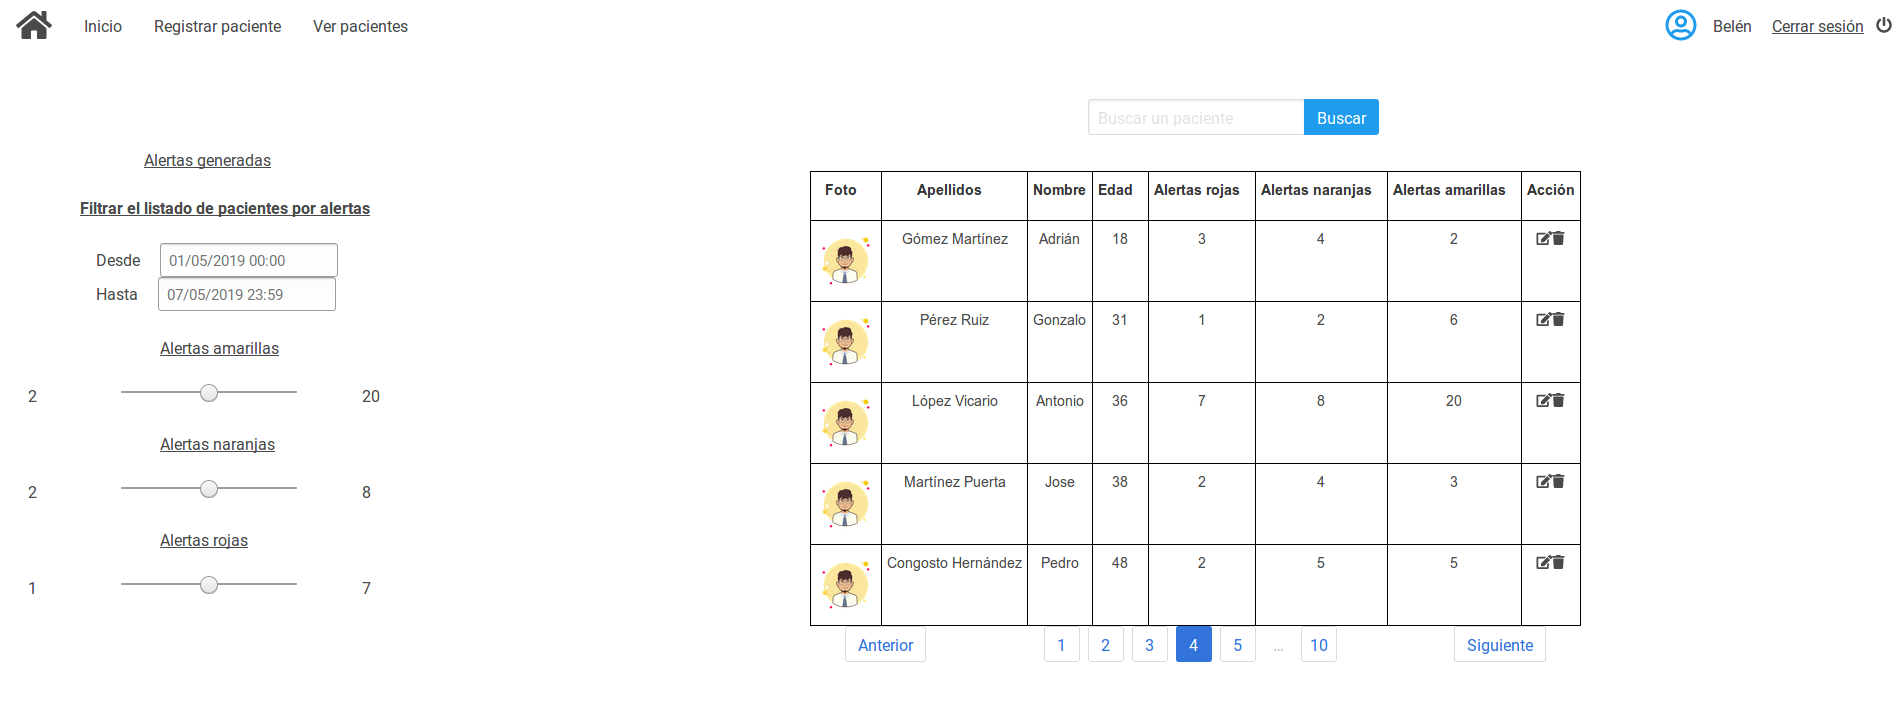
\includegraphics[height=7.5cm, width=\textwidth]{Imagenes/anxA17.png}
    \caption[Mockup de la pantalla principal de la web]{Mockup de la pantalla principal de la web}
    \label{fig:c4:mockup26}
\end{figure}

\paragraph{}
En las figuras~\ref{fig:c4:mockup27} y~\ref{fig:c4:mockup28} se puede ver la pantalla en la que aparecería el resumen de cada paciente mediante una gráfica y una tabla de formato acordeón a continuación con información detallada de cada uno de los estados del episodio por los que ha pasado el paciente.

\begin{figure}[!htbp]
    \centering
    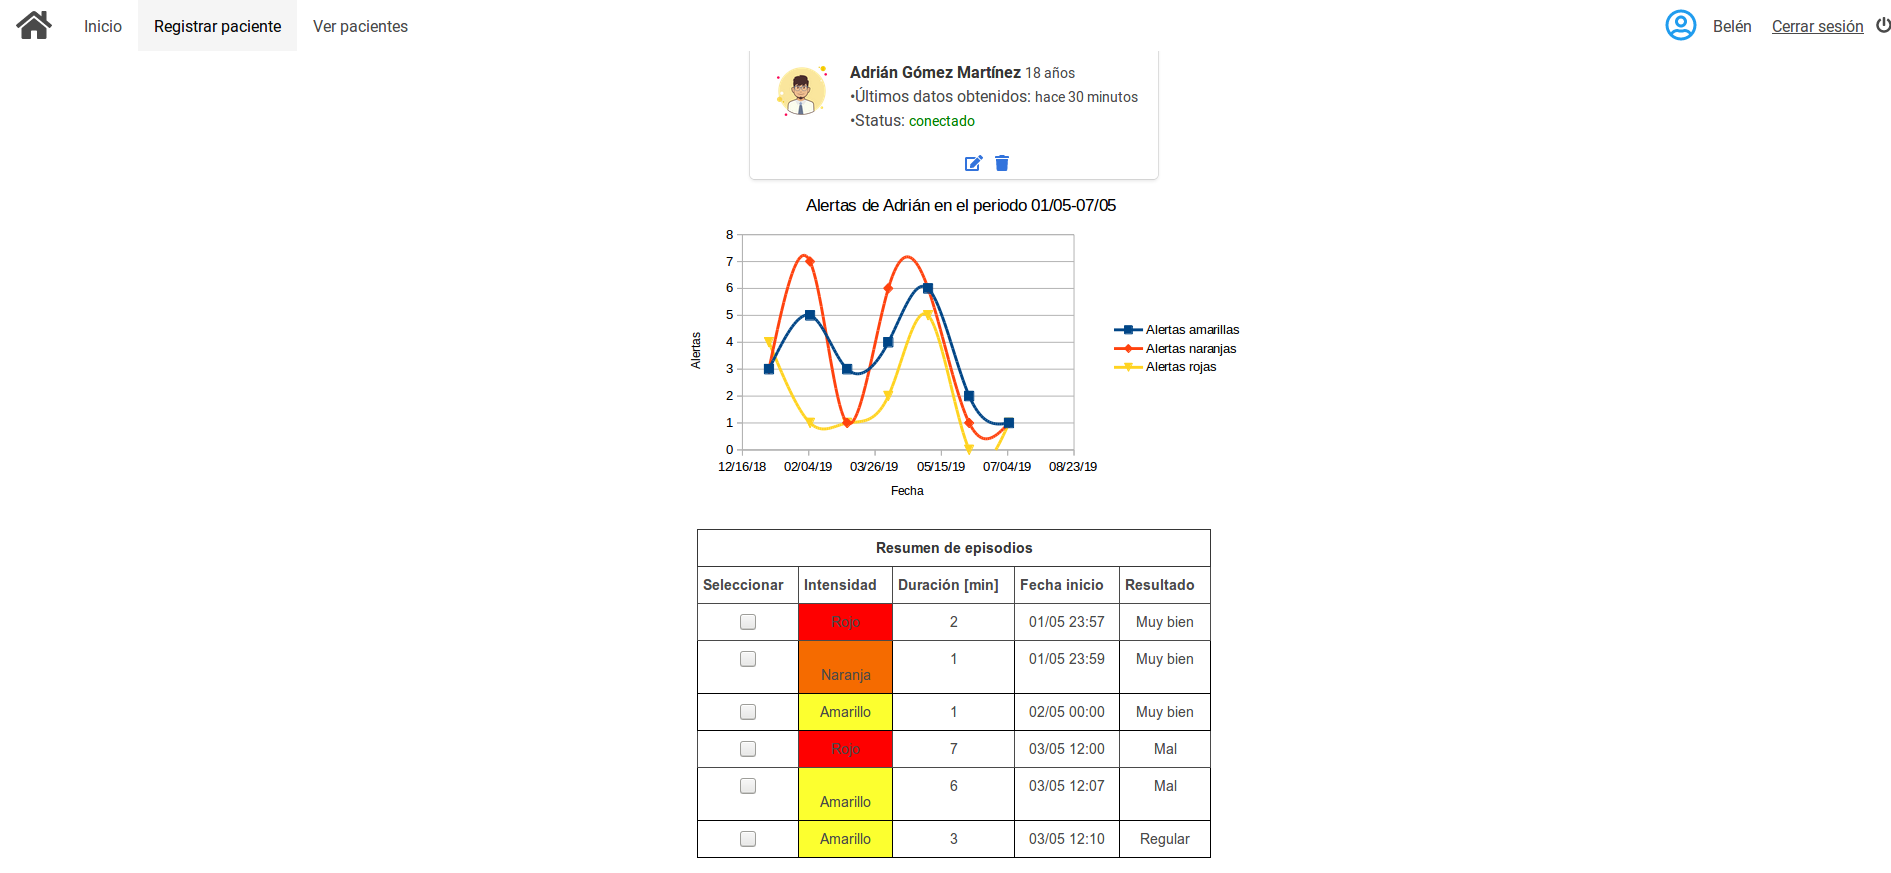
\includegraphics[height=7.5cm, width=\textwidth]{Imagenes/anxA18.png}
    \caption[Mockup de la pantalla para ver los episodios (I/II)]{Mockup de la pantalla para ver los episodios (I/II)}
    \label{fig:c4:mockup27}
\end{figure}

\begin{figure}[!htbp]
    \centering
    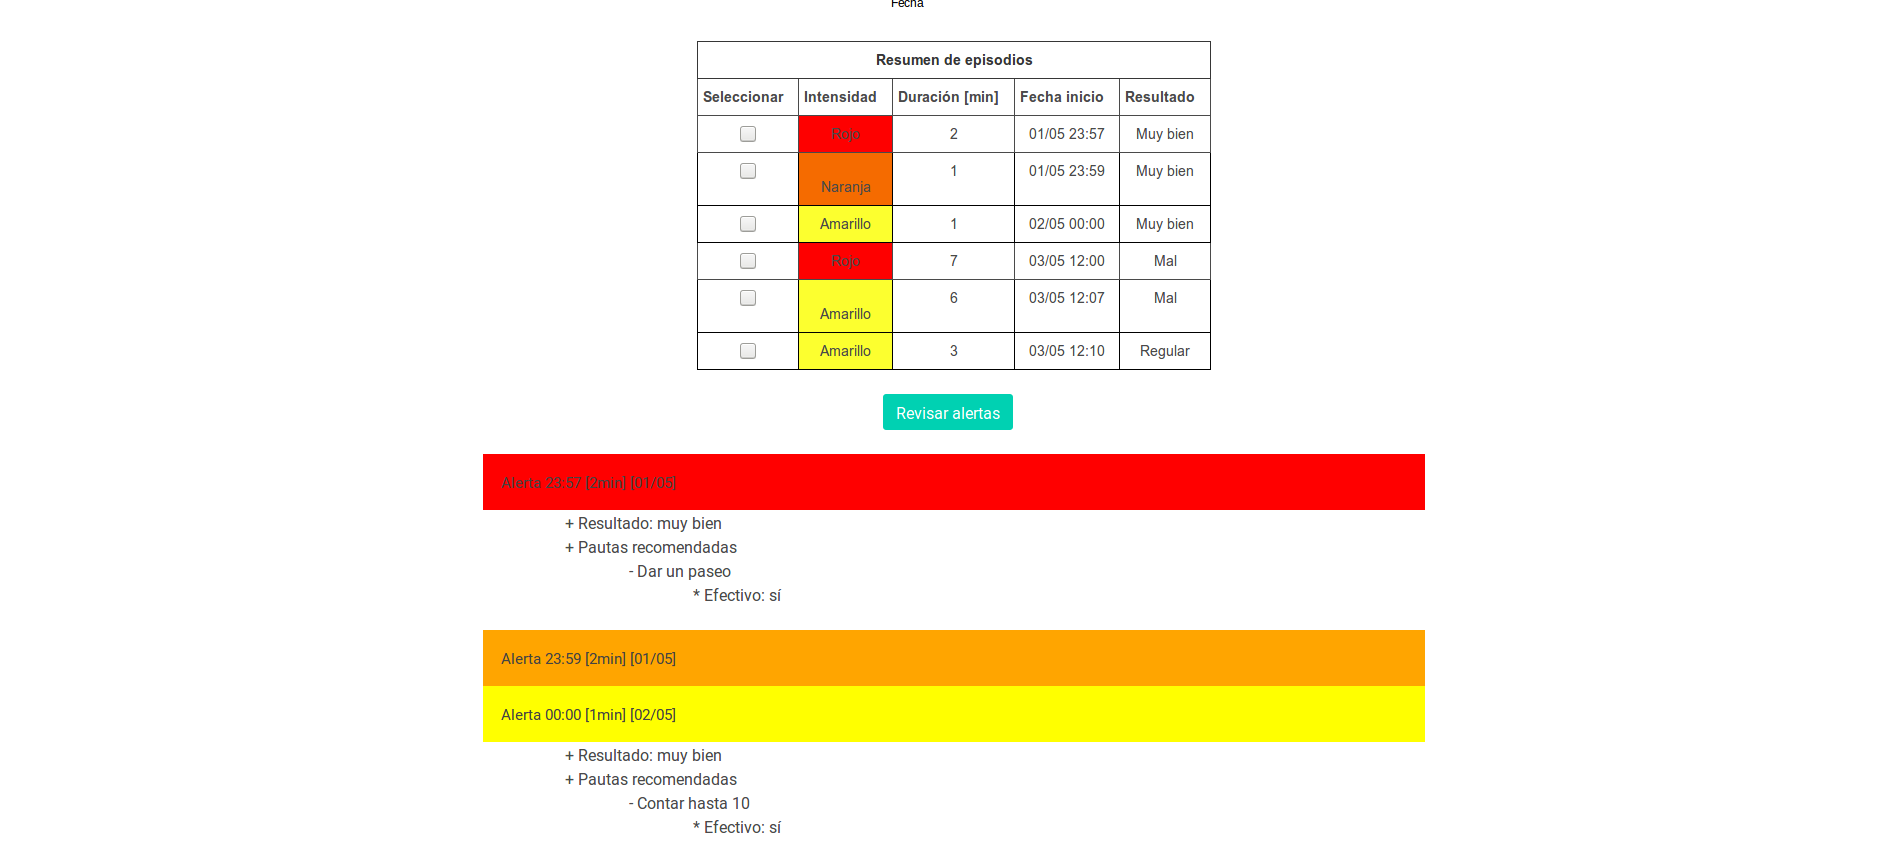
\includegraphics[height=7.5cm, width=\textwidth]{Imagenes/anxA19.png}
    \caption[Mockup de la pantalla para ver los episodios (II/II)]{Mockup de la pantalla para ver los episodios (II/II)}
    \label{fig:c4:mockup28}
\end{figure}

\paragraph{}
En la figura ~\ref{fig:c4:mockup25} se puede ver la implementación de la pantalla ~\ref{fig:c4:mockup5} en la versión en la que las pautas están separadas por el nivel de activación.

\begin{figure}[!htbp]
    \centering
    %width=3cm, height=3cm
    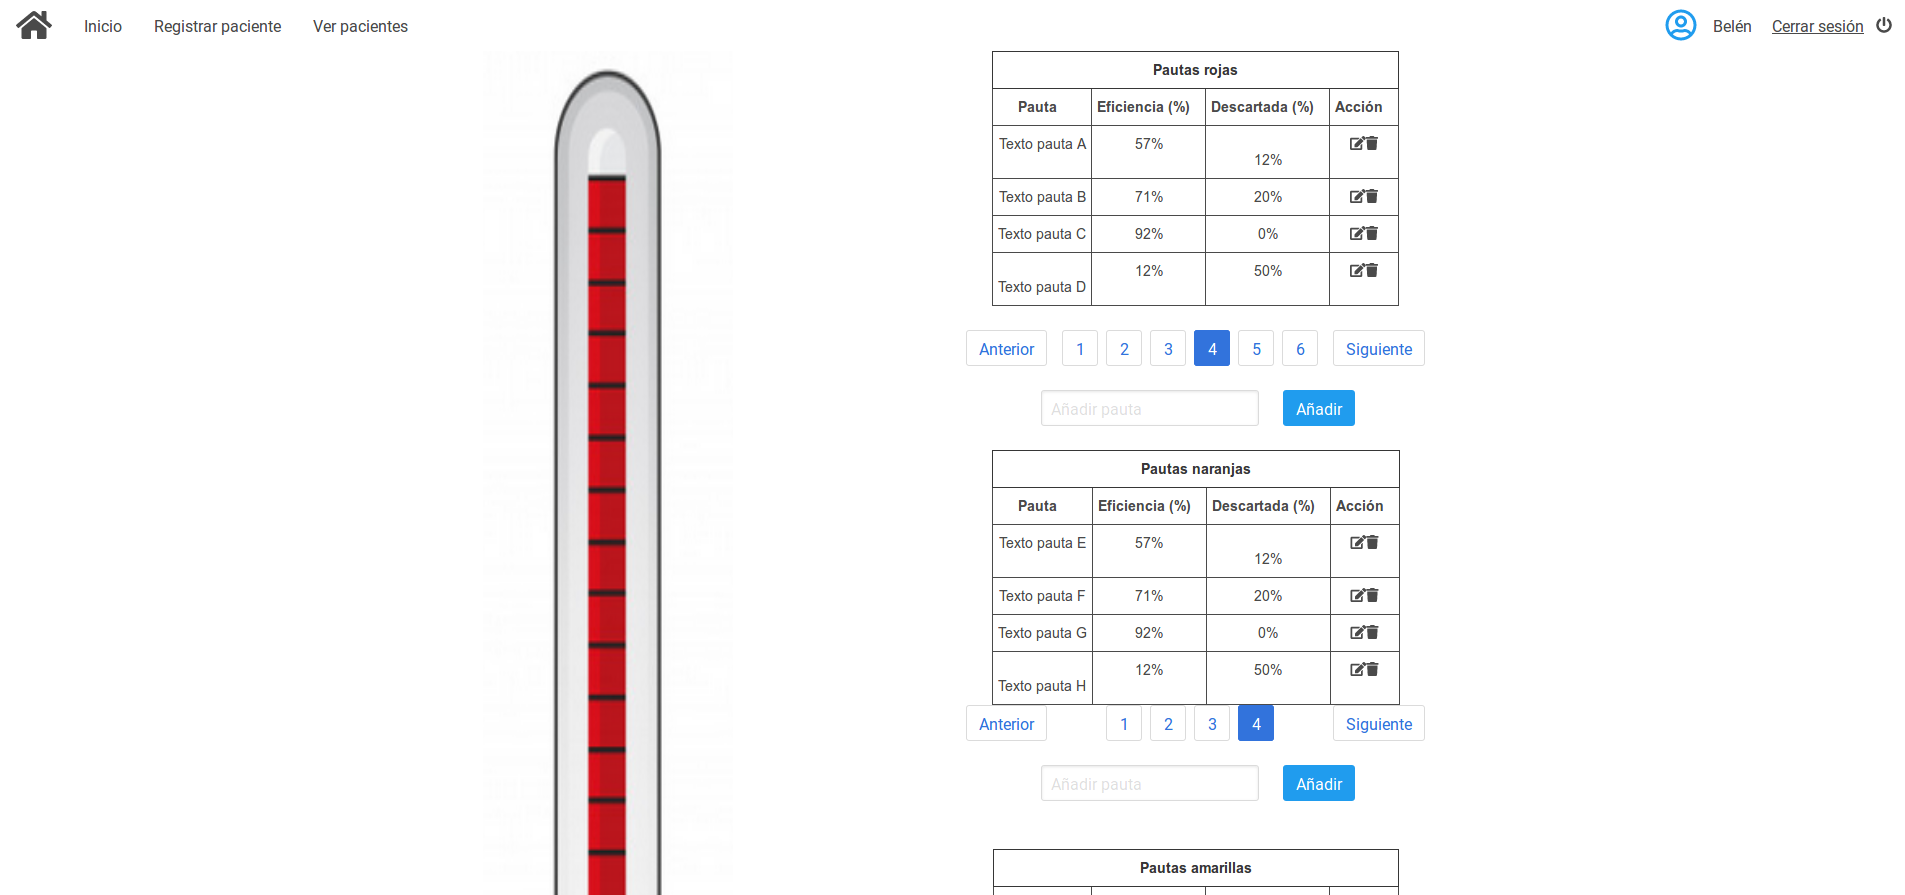
\includegraphics[height=7.5cm, width=\textwidth]{Imagenes/anxA20.png}
    \caption[Mockup de la pantalla para ver las pautas]{Mockup de la pantalla para ver las pautas}
    \label{fig:c4:mockup31}
\end{figure}

\paragraph{}
Tras la reunión con la terapeuta, los puntos que se sacaron en claro fueron los siguientes:

\begin{itemize}
    \item Las pantallas de las figura~\ref{fig:c4:mockup17} y~\ref{fig:c4:mockup18}  siguen teniendo en las tablas y en la gráfica alertas en lugar de eventos, por lo que los elementos que aparezcan en la web deben ser el conjunto de eventos del paciente en el que, al seleccionar algún episodio concreto, se pueda ver la información detallada de dicho episodio.
    \item La tabla de la figura~\ref{fig:c4:mockup18} debe ser interactiva. Se insiste en emular el diseño de los desfibriladores. La tabla de la figura~\ref{fig:c4:mockup19} que aparece debajo indicando las pautas seguidas en los distintos momentos es correcta, pero en el diseño final tiene que ser más detallada.
    \item La pantalla de la figura~\ref{fig:c4:mockup31} es una representación adecuada de las pautas almacenadas.
    \item Se echa en falta definir la pantalla en la que se añaden las pautas de cada paciente. En estas es necesario crear un sistema para poder heredar pautas de manera grupal para, a partir del paquete de pautas que se ha heredado, poder personalizarlas para cada paciente.
\end{itemize}

%TODO: esto probablemente acabe en otra sección mucho más detallada en la que se expliquen todos los aspectos técnicos de la solución final.
\section{Implementación}
\label{sec:c4:impl}
\paragraph{}
La pulsera es un dispositivo IOT que obtendrá las sensorizaciones del paciente cada [TODO] segundos. Concretamente, obtendrá los datos de sudoración, [TODO: constantes fisiológicas medidas]. Para ello, se ha elegido el modelo [TODO: modelo y descripción del modelo de la pulsera haciendo referencia a la comparación de pulseras del estado del arte].

\paragraph{}
Estas sensorizaciones se enviarán por BLE al dispositivo móvil con sistema operativo Android del paciente. La conexión será gestionada mediante una app creada para este proyecto, que irá guardando las sensorizaciones en una base de datos local de SQLite. La base de datos local estará encriptada con el algoritmo [TODO: rellenar cuando termine la app] para evitar dos posibles ataques: por un lado, si el paciente tiene el móvil \textit{rooteado} y la base de datos no está encriptada, si se instalase una aplicación maligna, esta podría acceder a los datos de la base de datos. Por otro, aunque el paciente no tuviera el móvil \textit{rooteado}, es necesario prevenir que estos datos se vieran expuestos si una tercera persona no autorizada tuviera acceso físico al mismo por ejemplo porque hubiese dejado desatendido su dispositivo temporalmente o le robasen el dispositivo.

\paragraph{}
En las aplicaciones móviles es crucial optimizar al máximo el uso de recursos para evitar que la aplicación creada interfiera con el normal funcionamiento del dispositivo ralentizándolo, consumiendo muchos datos o almacenando datos innecesarios. En esta línea, la aplicación borrará las sensorizaciones guardadas en local una vez hayan sido transformadas en episodios. Un episodio es un conjunto de sensorizaciones del paciente que muestran la transición del mismo desde que está calmado, se detecta la ira y vuelve al estado inicial. Como en el trabajo una vez transformada las sensorizaciones en posibles episodios esta información no es útil, se borra en cuanto se ha realizado esta conversión.

\paragraph{}
[TODO: expicar cuando esté la app de Android cómo se transforman las sensorizaciones en episodios.]

\paragraph{}
Por otro lado, los episodios del paciente sí persisten en la base de datos local de SQLite del dispositivo Android del paciente, ya que éste podrá acceder al archivo histórico de sus episodios para poder ver su progreso. Cada cinco minutos, se realizará una comunicación con el servidor para indicarle si en los últimos cinco minutos se han producido episodios de ira, y en cuyo caso se explicitará el episodio.

\paragraph{}
Como se ha comentado al principio de esta sección, cuando se detecte que el paciente pueda estar sufriendo un episodio de ira, se le proveerán de pautas en tiempo real que puedan ayudar a rebajar su nivel de ira. Las pautas recomendadas en ese momento podrán ser descartadas por el paciente y podrá añadir comentarios sobre la idoneidad de las mismas. Las pautas que aparezcan y la manera en la que el paciente interaccione con las mismas (si introduce comentarios, si las descarta, si han sido efectivas a la hora de rebajar el nivel de ira) será registrado en la base de datos local ya que esta información ayudará luego al terapeuta a ajustar mejor las pautas más adecuadas para cada paciente.

\paragraph{}
Estos datos se enviarán al servidor en formato JSON mediante el protocolo AMQP. Este es un protocolo de comunicación específicamente pensado para dispositivos IOT debido a su bajo consumo de recursos. Esta información estará cifrada usando el protocolo SSL para evitar robos de información sensible del paciente mediante técnicas de \textit{sniffing} o ataques de \textit{Man in the middle}.

\paragraph{}
Una vez llegan los datos de los posibles episodios y sus correspondientes pautas al servidor de AMQP, estos datos serán desencriptados y se persistirán en una base de datos de Mongo. El servidor contará con dos bases de datos: una base de datos SQLite que únicamente almacenará los credenciales de los terapuetas para acceder a la web y una base de datos de Mongo en el que se almacenará el resto de la información.

\paragraph{}
En la web el terapeuta podrá añadir nuevos pacientes, asociar pautas a pacientes en función de la intensidad de ira que se detecte y ver el histórico de episodios de cada paciente. Así, según las veces que se haya descartado una pauta, la efectividad de la misma o los comentarios de cada paciente, podrá modificar o eliminar la pauta para uno o más pacientes. Esto también sirve para poder comentar con el paciente los distintos episodios de ira que ha sufrido teniendo un registro histórico que pueda servir como referencia para guiar la terapia.